% !TeX root = 00General.tex
\thispagestyle{standard}
\pagestyle{standard}
\chapter{Network Reconnaissance}

\section{Network Ping Sweep}

In this part information about hosts in a connected network is gathered.
With the help of the Kali VM a \texttt{nmap} Ping Sweep command is executed to gather information of the connected devices within the network of the given IP.\\
\texttt{nmap -sP 172.16.1.*}

The information gathered are the IP address of the connected device and his MAC address.

\begin{figure}[H]
	\centering
	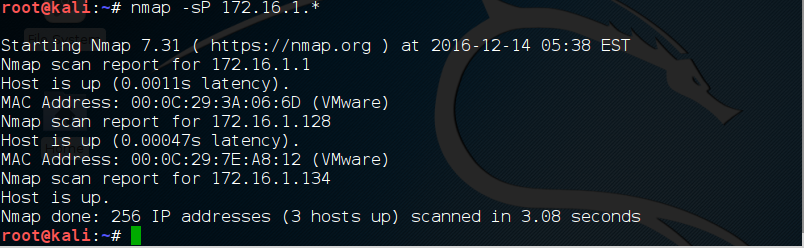
\includegraphics[width=0.9\textwidth]{img/2_1_Network_Ping_Sweep_Kali.PNG}
	\caption{Network Ping Sweep with Kali VM}
	\label{img:network ping sweep}
\end{figure}

After the switch to the Ubuntu VM we can analyze the Wireshark trace we started in first place. The trace shows that the \texttt{nmap} Ping Sweep command executes an \ac{ARP}-request on every host on the given IP network range. If a host is available he answers with his MAC address.

\textit{Advanced:}\\
If a system detects a certain amount of new \ac{ARP}-requests on every host system in a network then this could be a sign for an intrution. Since \ac{ARP} is a stateless protocol, hosts in the network can be compromised by spoofing with falsified IP-MAC pairs.

\section{OS Detection}

Informations about a specific host in the network are gathered. With the help of the Kali VM an OS detection command is executed.\\
\texttt{nmap -O -v 172.16.1.X}
\newpage
The gathered informations are:
\begin{itemize}  
\item Open ports
\item MAC address
\item Device type
\item The running operation system 
\item The network distance to the host (in hops)
\item TCP Sequence Prediction
\end{itemize}
With these information further steps can be planned and executed to compromise this specific host system.

\begin{figure}[H]
	\centering
	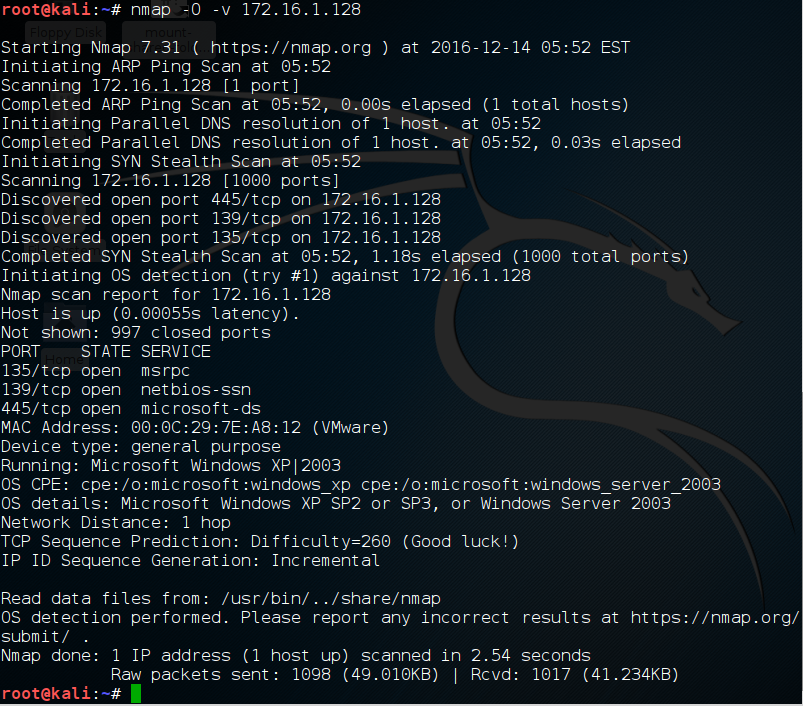
\includegraphics[width=0.9\textwidth]{img/2_2_OS_Detection_Kali.PNG}
	\caption{OS detection nmap command with Kali VM}
	\label{img:os detection kali}
\end{figure}

\section{Email Sniffing}

In this part Wireshark is used to listen to packets of the \ac{POP3} protocol. After receiving the authentication packets from the mail server a few \ac{POP3} packages can be found. One of the packets contains a character sequence which is base64-encoded (e.g. \texttt{"AHJla3RvcgByZWt0b3I"}). This sequence can then be decoded with an external decoder to the username and password of the client which tried to authenticate on the mail server (in this example it is \texttt{"rektor rektor"}).

After sending an receiving an email from the mail server an \ac{SMTP} packet can be found where the sender, receives, subject and the email text is shown in plaintext. When the attack is performed on the Kali VM it shows the same results (base64-decoded authentication and plaintext \ac{SMTP} packet).

\textit{Advanced:}\\
To let this attack be successful an non secured transport protocol need to be used and the used \ac{SMTP} needs to be in plaintext.
One counter-measure is the use of \ac{SSL} for \ac{SMTP} connections. This raises another problem. By default, all \ac{SMTP} servers use port 25. But if you use \ac{SSL} on port 25, non-\ac{SSL} will not be able to connect through that port. And if you use a nonstandard port number, other servers will not be able to find your server.
Another counter-measure is the use of \ac{TLS} for an \ac{SMTP} connection. Each end of the connection can choose to authenticate the other, or the \ac{TLS} connection can be used purely for privacy. (http://windowsitpro.com/exchange-server/securing-smtp-email-traffic)